\documentclass[12pt]{article}
\usepackage[utf8]{inputenc}
\usepackage{mathtools}
\usepackage{cancel}
\usepackage[margin=1.0in]{geometry}
\usepackage[margin=1.0in]{caption}
\usepackage[table]{xcolor}
\usepackage{gensymb}
\usepackage{graphicx}
% for å få inn source code
\usepackage{amssymb} 
\usepackage{amsmath} 
\usepackage[utf8]{inputenc} 
\usepackage[norsk]{babel} 
\usepackage[T1]{fontenc}
\usepackage{listings}

\title{IFYT1001 Lab:\\ Målig av akselerasjon til forskjellige legemer på skråplan\newline}

\author{
  Brand, Nicolai\\
  \and
  Gran, Callum\\
  \and
  Gützkow, Carl\\
  \and
  Hansen, Eilert Werner\\
  \and
  Kvamme, Brage\\
  \and
  Gudvangen, Trym\\
}
\date{8. mars 2022}

\newcommand{\uu}[1]{\underline{\underline{#1}}}

\begin{document}

\maketitle
\smallskip
\section{Hensikt}

\paragraph{Hensikten med dette forsøket var å bestemme akselerasjonen fra forskjellige legemer som ruller uten å gli nedover et skråplan.
Dette forsøket viste hvordan formlene som læres i faget fungerer i praksis, samt viste det usikkerheten til resultatene i forhold til det som var forventet.}

\section{Teori}

\paragraph{Figuren under viser kreftene som virker på et legeme som ruller ned et skråplan. Videre skal det utledes et uttryk for den translatoriske akselerasjon i x retning $a_x$ gitt vinkelen $\beta$ og konstanten $c$ som sier noe om hvordan massen til et legeme er distribuert}

\newpage

\begin{figure}[htp]
    \centering
    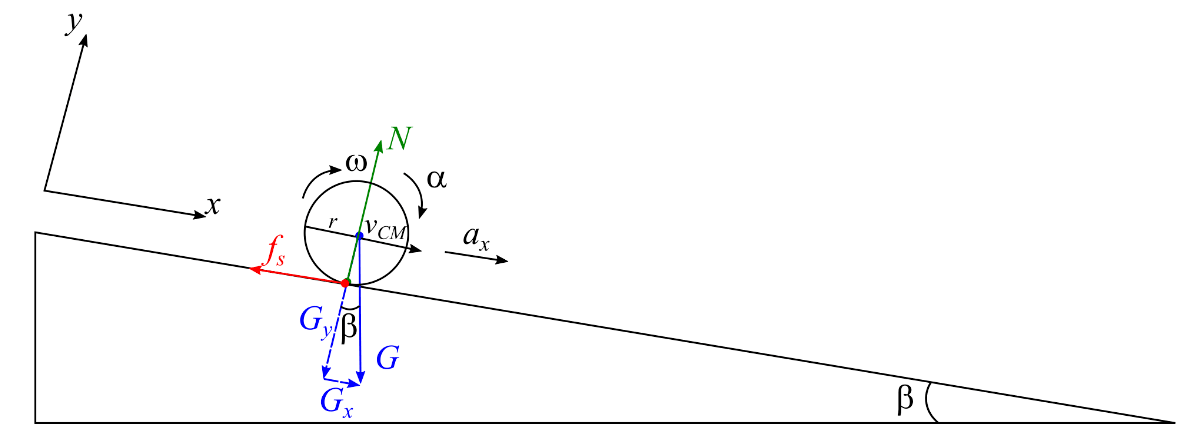
\includegraphics[width=12cm]{fig_kok.png}
    \caption{To dimensjonal figur av oppsettet. Hentet fra https://home.phys.ntnu.no/fyslabing/assets/labhefte.pdf (24.03.2022).}
    \label{fig:oppsettfig}
\end{figure}

\paragraph{Newtons 2. lov gir:}

\begin{align}
    \sum F_x &= ma_x \nonumber \\
    G_x - f_s &= ma_x \nonumber \\
    m g sin \beta - f_s &= m a_x
\end{align}

\paragraph{Friksjonskraften skaper et dreiemoment. Newtons 2. lov for rotasjonsbevegelse gir:}

\begin{align}
    \sum \tau &= I\alpha \nonumber \\
    f_s r &= I \alpha
\end{align}

\paragraph{Sammenhengen mellom rotasjonsbevegelse og translatoriskbevegelse gir:}

\begin{align}
    a_x = \alpha r, \hspace{10pt} v_{CM} = \omega r
\end{align}

\begin{align}
    c = \frac{K_{rotasjon}}{K_{translasjon}} = \frac{\frac{1}{2} I \omega^2}{\frac{1}{2} M v_{CM}^2}
\end{align}

\paragraph{Oppgaven var å bruke formlene over for å finne en formel for å finne $a_x$.}

\begin{align*}
    \textbf{Omformulerer (1)} \\
    f_s &= m g sin \beta - m a_x \\
    \textbf{(1) inn i (2)} \\
    (m g sin \beta - ma_x) \cdot r &= I \alpha \\
    r m g sin \beta  - r m a_x &= I \alpha \\
    \textbf{Bruker (3) for å bytte ut $\alpha$} \\
    r m g sin \beta  - r m a_x &= I \frac{a_x}{r} \\
    r m g sin \beta &= a_x (I \frac{1}{r} + r m) \\
    a_x &= \frac{r m g sin \beta}{I \frac{1}{r} + r m} \\
    a_x &= \frac{r m g sin \beta}{r m ( \frac{I}{r^2 m} + 1)} \\
    a_x &= \frac{g sin \beta}{ \frac{I}{r^2 m} + 1} \\
    a_x &= \frac{g sin \beta}{ \frac{I \cdot w^2}{r^2 m \cdot w^2} + 1} \\
    \textbf{Bruker (3) for å bytte ut $\omega$} \\
    a_x &= \frac{g sin \beta}{ \frac{I \cdot w^2}{r^2 m \cdot (\frac{v_{CM}}{r})^2} + 1} \\
    a_x &= \frac{g sin \beta}{ \frac{I \cdot w^2 \cdot \frac{1}{2}}{m v_{CM}^2 \cdot \frac{1}{2}} + 1} \\
    \textbf{Bytter ut del av telleren med (4)} \\
    a_x &= \frac{g sin \beta}{ c + 1} \\
\end{align*}
Dette førte til at likningen over ble utledet. Dermed kan vi finne akselerasjonen (\(a_x\)) i x-retningen nedover skråplanet for et objekt som ruller uten å gli. Vi kan dermed konkludere at alerasjonen vil være avhengig av tyngdeakselerasjonen, vinkelen på helningen og konstanten c.

\newpage
\section{Metode}

\subsection{Utstyr}
\begin{itemize}
    \item Datamaskin med Pasco CAPSTONE
    \item Et skrått plan på 1 meter eller lengre
    \item Et instrument for å måle lengde
    \item En Pasco avstandsmåler
    \item Diverse gjenstander for å skape høyde slik at vinkelen er ca. 9\degree
    \item 2 ulike rullende objekter
\end{itemize}

\begin{figure}[htp]
    \centering
    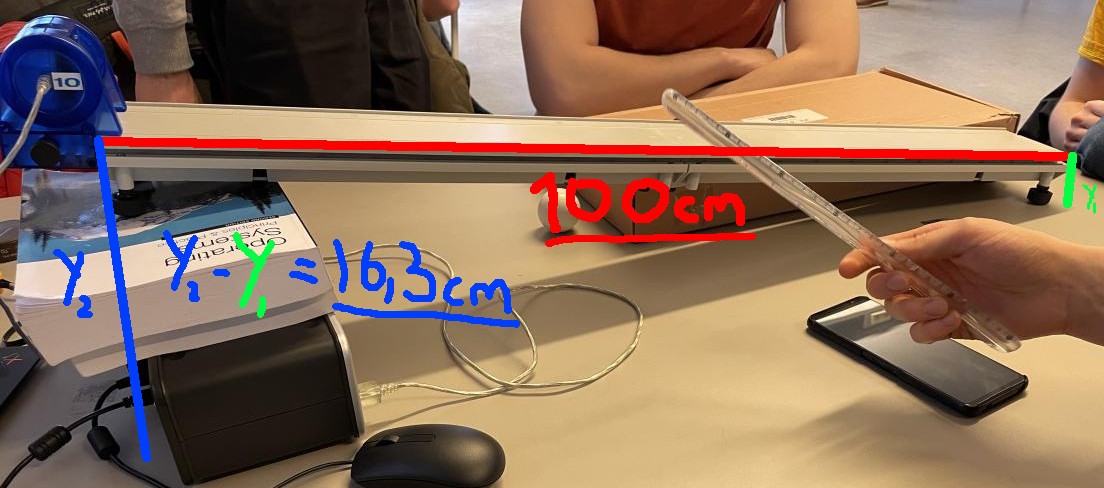
\includegraphics[width=14cm]{oppsett.jpg}
    \caption{Bilde av oppsettet}
    \label{fig:oppsett}
\end{figure}

\subsection{Utførelse}
\paragraph{Sett opp et skråplan med en avstandsmåler på toppen. Denne avstandsmåleren ble konfigurert til å måle på 50 hz. Ved hjelp av en telefon med en applikasjon med måleverktøy ble helningsvinkelen målt til $9,4\degree$. Hypotenusen ble målt til 100 cm og høyden ble målt til 16,3 cm. Ved hjelp av trigonometri ble det funnet en verdi for helningsvinkelen for å sjekke at den første målingen var pålitelig.}

\paragraph{Merk at det ikke kan brukes spesialtegn i LaTeX matte, så derfor står det \newline engelske begreper.}
\begin{align*}
    \sin(\alpha) &= \frac{height}{hypotenuse} \\
    \alpha &= \arcsin(\frac{height}{hypotenuse}) \\
    \alpha &= \arcsin(\frac{16.3 cm}{100 cm}) = 9.38107.. cm \approx 9.38 \degree \\
\end{align*}

\paragraph{Vinkelen som ble målt og den utregnede vinkelen var $9.4\degree$ når det brukes to gjeldende siffer. Videre brukes verdien 9.38 \degree som helningsvinkel ettersom antall gjeldende siffer er tre.}

Videre ble to rullende objekter valgt for å rulle ned skråplanet. \\


\begin{figure}[htp]
    \centering
    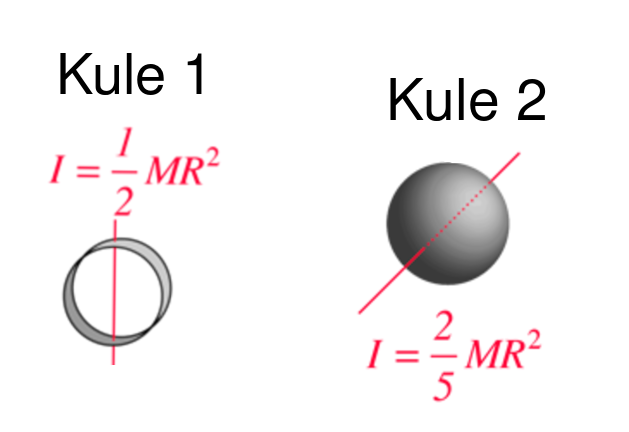
\includegraphics[width=8cm]{figur1.png}
    \caption{Kulene sin form og deres dreiemoment}
    \label{fig:kule}
\end{figure}

\paragraph{Ved å bruke linjal ble det funnet at radiusen til både $kule_1$ og $kule_2$ var $2,5 cm$. Fra figuren kan man se at formen på kulene gjør at de får et ulikt treghetsmoment. Konstanten foran $MR^2$ i uttrykket for treghets moment kan kalles $c$. Denne verdien er knyttet til hvordan massen til en figur er distribuert. Ved hjelp av tabell kan en se at $kule_1$  får en $c$ på $\frac{1}{2}$ og $kule_2$ får en $c$ på $\frac{2}{5}$.}

\paragraph{Videre ble hver av kulene sluppet fra stillestående posisjon på toppen av skråplanet. Dette ble gjort fem ganger for hver kule. Deretter ble programmet PASCO Capstone brukt til å logge målingene fra avstandsmåleren. Ved hjelp av regresjon ble dataen omgjort til en andregradsfunksjon med konstantene A, B, og C. Verdiene for A, B og C ble beregnet utifra resultatene skrevet i seksjon \ref{sec:res}. Konstanten A representerer halvparten av akselerasjonen til legemets massesenter langs skråplanet. Dette er fordi regresjonen av avstandsmålingene gir en funksjon på formen $At^2+Bt+C$ som korrelerer med bevegelseslikningen $\frac{1}{2}at^2+v_0t$. I denne rapporten er verdiene for B og C ikke interessante, men en avgjørelse ble tatt for å ta de med uansett.}

For å regne ut usikkerheten ble et Python program skrevet. Kildekoden til programmet: \\
\resizebox{17cm}{!}{
    \lstinputlisting[language=Python]{std_dev.py}
}

\section{Resultater} \label{sec:res}

\paragraph{Usikkerhetene i resultatene kommer fra PASCO.}

%Resultat fra sylinder
\begin{table}[h]
    \centering
    \rowcolors{2}{gray!25}{white}
    \begin{tabular}{c|c|c|c|c|c}
        \rowcolor{gray!50}
        Sylindrisk ring & 1 & 2 & 3 & 4 & 5 \\
        \hline
        A & 0.51 & 0.589 & 0.449 & 0.491 & 0.428 \\
        A usikkerhet & 0.018 & 0.024 & 0.021 & 0.018 & 0.02 \\
        B & -0.356 & -0.291 & 0.00563 &	-0.035 & 0.0417 \\
        B usikkerhet & 0.051 & 0.053 & 0.048 & 0.039 & 0.049 \\
        C & 0.011 & 0.0385 & -0.104 & -0.0597 & -0.135 \\
        C usikkerhet & 0.034 & 0.028 & 0.026 & 0.02 & 0.029
    \end{tabular}
    \caption{Resultat fra sylindrisk kule (kule 1)}
    \label{tab:2}
\end{table}

% Resultater fra kule
\begin{table}[h]
    \centering
    \rowcolors{2}{gray!25}{white}
    \begin{tabular}{c|c|c|c|c|c}
        \rowcolor{gray!50}
        Kule & 1 & 2 & 3 & 4 & 5 \\
        \hline
        A & 0.777 & 0.86 & 0.746 & 0.722 & 0.732 \\
        A usikkerhet & 0.026 & 0.046 & 0.046 & 0.023 & 0.015 \\
        B & -2.1 & -1.02 & -0.543 & 0.023 & 0.015 \\
        B usikkerhet & 0.1 & 0.1 & 0.086 & 0.053 & 0.029 \\
        C & 1.47 & 0.375 & 0.147 & 0.292 & 0.1 \\
        C usikkerhet & 0.098 & 0.057 & 0.039 & 0.03	& 0.014
    \end{tabular}
    \caption{Resultat fra kule (kule 2)}
    \label{tab:1}
\end{table}


\paragraph{Ved å sette inn målingene for $2 \cdot A$ i Python programmet vedlagt i seksjon 3.2 (Utførelse) gis det verdier for gjennomsnitt, standardavvik og standardfeil. Årsaken til at man må gange målingene for A med 2 er forklart i seksjon 3.2 (Utførelse).}

Sylindrisk ring (Kule 1) \\

Gjennomsnitt: $\bar{a_x}$ = $0.987 m/s^2$.\\
Standardavvik: $\delta a_x$ = $0.112 m/s^2$.\\
Standardfeil: $\delta \bar{a_x}$ = $0.05 m/s^2$.\\
Resultat: $\bar{a_x}$ \pm $\delta \bar{a_x}$ = $(0.987$ \pm $ 0.05)m/s^2$.\\

Kule (Kule 2) \\
Gjennomsnitt: $\bar{a_x}$ = $1.54 m/s^2$.\\
Standardavvik: $\delta a_x$ = $0.125 m/s^2$.\\
Standardfeil: $\delta \bar{a_x}$ = $0.056 m/s^2$.\\
Resultat: $\bar{a_x}$ \pm  $\delta \bar{a_x}$ = $(1.54$ \pm $ 0.06)m/s^2$.\\

Fra seksjon 2 (Teori) ble følgende formelen utleddet:
\begin{align*}
        a_x &= \frac{g sin \beta}{ c + 1} \\
\end{align*}

Ved bruk av seksjon 3 (Metode) ble en verdi for helningsvinkelen $\beta$ og verdier for konstanten c regnet ut. 
\begin{align*}
    \beta = 9.38 \degree\\
    c_1 = \frac{1}{2}\\
    c_2 = \frac{2}{5}\\
\end{align*}

Derfra ble de teoretiske verdiene for $a_x$ til de to kulene regnet ut.

\begin{align*}
    Kule 1:
    a_x &= \frac{9.81 m/s^2 sin(9.38\degree)}{ \frac{1}{2} + 1} = 1.06 m/s^2 \\
    Kule 2:
    a_x &= \frac{9.81 m/s^2 sin(9.38\degree)}{ \frac{2}{5} + 1} = 1.14 m/s^2
\end{align*}


\section{Diskusjon}

\paragraph{Med dataene fra forsøkene, og med vekt på usikkerheten, ble resultatene som følger. Kule 1 hadde en akselerasjon på $\bar{a_x}$ \pm $\delta \bar{a_x}$ = $(0.987$ \pm $ 0.05)m/s^2$. Dette er en forskjell av $\Delta {a_x}$ = $(0.073 \pm 0.05)m/s^2$ fra den teoretiske akselerasjonen $a_x$ =  $1.06 m/s^2$. Kule 2 hadde en akselerasjon på $\bar{a_x}$ \pm $\delta \bar{a_x}$ = $(1.54$ \pm $ 0.06)m/s^2$. Igjen hadde dette en forskjell på $\Delta {a_x}$ = $(0.40 \pm 0.06)m/s^2$ fra den teoretiske akselerasjonen $a_x$ = $1.14 m/s^2$.}

\paragraph{Det var et avvik i det faktiske resultatet og resultatet det forventede resultatet. Dette kan komme av flere årsaker.}

\begin{itemize}
    \item Feilmåling av høyder som kan føre til feil utregning av vinkeler.
    \item Feil med måle aperatet i seg selv
    \item Feil bruk av måle aperatet som:
        \begin{itemize}
            \item Begynt målingen for tidlig
            \item Feil innstillinger på apparatet
        \end{itemize}
    \item Forskjeller i høyden til skråplanet på grunn av forskyvning.
    \item Tilføring av kraft til kulene i det de ble sluppet.
    \item Luftmotstand
    \item Forskjell i lufttetthet
    \item Skrå rulling (ikke rett linje som betyr lengre distanse).
    \item Regnefeil med kalkulator
\end{itemize}

\paragraph{Av feilkildene er det noen faktorer som har større påvirkning enn andre. Luftmotstanden og lufttetthet vil ha en ubetydelig effekt på grunn av hastighetene som ble oppnådd under forsøket. I tillegg var skråplanet nokså stabilt og det ble antagelig ingen store forskjeller. Apparatene som ble brukt var nokså enkle i bruk, dermed var det lav sannsynlighet at dette påvirket resultatet substansielt. Menneskelige feil var antageligvis der avviket kommer fra. Det var blant annet mulig at høyden og lengden ble målt feil. Tilføring av kraft til kulen kunne også gitt en merkbar endring i hastigheten dersom dette vil ha skjedd til en viss grad hver gang ballen ble sluppet. Om det var en regnefeil så betyr dette at resten av feilkildene ikke er gjeldende.}
\paragraph{
$Kule_2$ var formet som en kule og overflaten var polert. Under antagelsen at avstandsmåleren sender ut lys, og regner avstand ut i fra tiden det tar før lyset reflekteres fra kulen, kan en tenke seg en mulig forklaring til at avviket ble så stort. Ettersom objektet var kuleformet og polert kan en se for seg at lyset som reflekteres ikke går i en rett linje tilbake til avstandsmåleren. Dette kan føre til at avstandsmåleren ikke får en jevn tilførsel med reflektert lys som i effekt ikke gir et riktig resultat. Det er viktig å nevne at dette bare er konjektur og et forslag til en forklaring.}


\section{Konklusjon}

\paragraph{
    Hensikten med dette forsøket var å regne ut akselerasjonen til to forskjellige legemer for deretter å sammenligne dette met akselerasjon fra målinger. Det viste seg at den faktiske verdien og den målte vedrien til $kule_1$ er bare omlag $7\%$ ulike. I betraktning av mulige feilkilder nevnt i 5 (Diskusjon) er dette et forventet avvik. Ser en på $kule_2$ er forskjellen mellom den faktiske verdien og den målte verdien omlag $30\%$. Dette er et større avvik en det som er forventet ut i fra feilkildene. I 5 (Diskusjon) blir mulige årsaker på dette nevnt.}
    
\section{Videre utforskning}

\paragraph{
    Videre vil en person som eksperimenterer med akselerasjonen av legemer kanskje utforske med forskjellige vinkler. En rekke vinkler kan gi interessante resultater når man sammenligner hvordan de passer med modellen. Det må bemerkes at en ny usikkerhet (vinkelusikkerhet) må tas mer i betraktning.}

\paragraph{
    I tillegg, så kan man eksperimentere med forskjellige typer flater som blir brukt som skråplanet. Hvis legemet opplever større friksjon mot skråplanet så kan dette føre til mindre glidning og et annerledes resultat. }

\end{document}
